%%%%%%%%%%%%%%%%%%%%%%%%%%%%%%%%%%%%%%%%%%%%%%%%%%%%%%%%%%%%%%%%%%%%%%%%%%%%%%%%
% ARTIGO CIENTÍFICO — modelo abnTeX2 (formato "article")
% Conformidade com ABNT: NBR 14724, NBR 6023, NBR 6024, NBR 6028, NBR 10520.
%
% Como compilar (Overleaf): Menu > Compiler = pdfLaTeX. A sequência é
%   pdfLaTeX -> BibTeX -> pdfLaTeX -> pdfLaTeX  (o Overleaf faz isso ao
%   clicar em "Recompile"; se as citações saírem como [?], recompile de novo).
%
% Edite APENAS o conteúdo. Os arquivos abntex2.cls, abntex2cite.sty e
% abntex2-alf.bst NÃO precisam ser editados.
%%%%%%%%%%%%%%%%%%%%%%%%%%%%%%%%%%%%%%%%%%%%%%%%%%%%%%%%%%%%%%%%%%%%%%%%%%%%%%%%

\documentclass[
	article,			% formato de artigo (seções em vez de capítulos)
	11pt,				% tamanho da fonte
	oneside,			% impressão só frente
	a4paper,			% tamanho do papel
	% -- opções do babel --
	english,			% idioma adicional (resumo em inglês)
	brazilian,			% idioma principal do documento
	sumario=tradicional
	]{abntex2}

% ---------------------------------------------------------------------------
% PACOTES
% ---------------------------------------------------------------------------
\usepackage[utf8]{inputenc}		% acentuação (UTF-8)
\usepackage[T1]{fontenc}		% codificação das fontes
\usepackage{lmodern}			% fonte Latin Modern
\usepackage{indentfirst}		% indenta o primeiro parágrafo de cada seção
\usepackage{graphicx}			% figuras
\usepackage{xcolor}			% cores
\usepackage{microtype}			% melhorias de justificação
\usepackage{amsmath,amssymb}		% matemática
\usepackage{booktabs}			% linhas de tabela mais elegantes
\usepackage{array}
\usepackage{multirow}
\usepackage{longtable}
\usepackage{listings}			% blocos de código
\usepackage{url}

% ---- Citações e referências padrão ABNT (autor-data) ----
\usepackage{hyperref}
\usepackage[brazilian,hyperpageref]{backref}
\usepackage[alf,abnt-emphasize=bf,abnt-etal-cite=3,abnt-etal-list=0]{abntex2cite}

% Configuração do backref (mostra em que página cada referência foi citada)
\renewcommand{\backrefpagesname}{Citado na(s) página(s):~}
\renewcommand{\backref}{}
\renewcommand*{\backrefalt}[4]{%
	\ifcase #3 %
		(Nenhuma citação no texto.)%
	\or
		(Citado na página #2.)%
	\else
		(Citado #3 vezes nas páginas #2.)%
	\fi}

% Cores dos links (discretas)
\definecolor{azulref}{RGB}{0,80,160}
\hypersetup{
	colorlinks=true,
	linkcolor=black,
	citecolor=azulref,
	urlcolor=azulref,
	pdftitle={Reconhecimento de padroes de falhas em etiquetas de codigos de barras},
	pdfauthor={Saymon Coppi de Oliveira Silva},
	pdfsubject={Visao computacional e orquestracao multiagente},
	pdfkeywords={codigo de barras, visao computacional, ADK, defeitos de impressao}
}

% ---- Estilo dos blocos de código ----
\definecolor{codebg}{gray}{0.96}
\definecolor{codecomment}{RGB}{0,120,0}
\definecolor{codestring}{RGB}{160,0,120}
\definecolor{codekw}{RGB}{0,0,180}
\lstset{
	basicstyle=\ttfamily\footnotesize,
	backgroundcolor=\color{codebg},
	keywordstyle=\color{codekw}\bfseries,
	commentstyle=\color{codecomment}\itshape,
	stringstyle=\color{codestring},
	numbers=left, numberstyle=\tiny\color{gray}, numbersep=7pt,
	breaklines=true, showstringspaces=false, frame=single,
	rulecolor=\color{gray!50}, captionpos=b, tabsize=2, columns=fullflexible,
	literate=%
		{á}{{\'a}}1 {é}{{\'e}}1 {í}{{\'i}}1 {ó}{{\'o}}1 {ú}{{\'u}}1
		{Á}{{\'A}}1 {É}{{\'E}}1 {Í}{{\'I}}1 {Ó}{{\'O}}1 {Ú}{{\'U}}1
		{à}{{\`a}}1 {â}{{\^a}}1 {ê}{{\^e}}1 {ô}{{\^o}}1 {ç}{{\c c}}1
		{ã}{{\~a}}1 {õ}{{\~o}}1 {Ç}{{\c C}}1 {Ã}{{\~A}}1 {Õ}{{\~O}}1
}

% ---------------------------------------------------------------------------
% DADOS DO TRABALHO  >>> EDITE AQUI <<<
% ---------------------------------------------------------------------------
\titulo{Reconhecimento de padrões de falhas em etiquetas de códigos de barras: um sistema de visão computacional com orquestração multiagente}

% Título em inglês (obrigatório no modelo de artigo abnTeX2: é impresso abaixo do título)
\tituloestrangeiro{Recognition of failure patterns in barcode labels: a computer vision system with multi-agent orchestration}

\autor{Saymon Coppi de Oliveira Silva\thanks{Universidade Federal de São Paulo
	(Unifesp), Instituto de Ciência e Tecnologia. Programa de Pós-Graduação em
	Ciência da Computação. Disciplina: Visão Computacional (cód.~2587), Prof. Dr.
	Fabio Augusto Menocci Cappabianco. E-mail: \texttt{saymoncoppi@gmail.com}.}}

\local{São José dos Campos}
\data{2026}

% Logo da instituição no topo da 1ª página (antes do título) — hook do memoir
\renewcommand{\maketitlehooka}{%
	\begin{center}
		
\includegraphics[width=5cm]{figuras/unifesp.png}
	\end{center}
	\vspace{0.4cm}%
}

% ===========================================================================
\begin{document}

\selectlanguage{brazilian}
\frenchspacing

% Título, autor e nota de rodapé de filiação
\maketitle

% ---------------------------------------------------------------------------
% RESUMO (português) — NBR 6028: 150 a 500 palavras, parágrafo único,
% linguagem impessoal, sem citações.
% ---------------------------------------------------------------------------
\begin{resumoumacoluna}
A leitura confiável de códigos de barras depende da qualidade de impressão das
etiquetas, avaliada por normas como a ISO/IEC 15416; contudo, os verificadores
certificados são caros e reportam apenas uma nota, sem indicar a causa física
do defeito nem a ação corretiva. Este trabalho propõe e desenvolve um sistema de
baixo custo que, a partir de uma imagem capturada por um dispositivo comum,
detecta defeitos típicos de impressão em etiquetas de códigos de barras e sugere
sua causa provável. A solução combina visão computacional --- uma rede neural
convolucional com \textit{backbone} leve, treinada por transferência de
aprendizado --- e orquestração multiagente com o \textit{Agent Development Kit}
(ADK), decompondo a tarefa em leitura/decodificação, estimativa de indicadores de
qualidade, detecção de defeitos físicos e diagnóstico de causa-raiz fundamentado
na documentação técnica do fabricante. O sistema é exposto por uma \textit{API}
única, consumida por um aplicativo Android e por uma interface web. A avaliação
prevista compara a arquitetura multiagente a uma abordagem monolítica,
quantificando o benefício da decomposição, e emprega um conjunto de dados
híbrido, com imagens reais de captura e defeitos de impressão gerados
sinteticamente de forma controlada e reprodutível. Espera-se demonstrar a
viabilidade de um apoio à decisão que vai além da nota, indicando causa provável
e correção sugerida.

\noindent
\textbf{Palavras-chave}: código de barras; qualidade de impressão; visão
computacional; aprendizado profundo; sistemas multiagentes.
\end{resumoumacoluna}

% ---------------------------------------------------------------------------
% ABSTRACT (inglês)
% ---------------------------------------------------------------------------
\begin{resumoumacoluna}[Abstract]
\begin{otherlanguage*}{english}
Reliable barcode reading depends on the print quality of the labels, which is
assessed by standards such as ISO/IEC 15416; however, certified verifiers are
expensive and report only a grade, without indicating the physical cause of the
defect or the corrective action. This work proposes and develops a low-cost
system that, from an image captured by an ordinary device, detects typical
printing defects in barcode labels and suggests their probable cause. The
solution combines computer vision --- a convolutional neural network with a
lightweight backbone, trained by transfer learning --- and multi-agent
orchestration with the Agent Development Kit (ADK), decomposing the task into
reading/decoding, quality-indicator estimation, physical-defect detection and
root-cause diagnosis grounded in the manufacturer's technical documentation. The
system is exposed through a single API, consumed by an Android application and by
a web interface. The planned evaluation compares the multi-agent architecture
with a monolithic baseline, quantifying the benefit of decomposition, and uses a
hybrid dataset with real capture images and printing defects generated
synthetically in a controlled and reproducible way. The expected outcome is to
demonstrate the feasibility of a decision-support tool that goes beyond the
grade, pointing to a probable cause and a suggested correction.

\noindent
\textbf{Keywords}: barcode; print quality; computer vision; deep learning;
multi-agent systems.
\end{otherlanguage*}
\end{resumoumacoluna}

% Sumário (opcional em artigos; comente as duas linhas abaixo se não quiser)
\tableofcontents*
\newpage

% ===========================================================================
\textual
% ===========================================================================

% ---------------------------------------------------------------------------
\section{Introdução}
% ---------------------------------------------------------------------------

\subsection{Contextualização}

Códigos de barras são a espinha dorsal da identificação automática de itens em
varejo, logística, saúde e manufatura. Uma etiqueta é lida dezenas de vezes ao
longo da cadeia --- na expedição, no transporte, no recebimento e no ponto de
venda --- e cada leitura pressupõe que a impressão preserve as proporções de
barras e espaços dentro de tolerâncias estreitas. Quando a impressão degrada, o
custo não é apenas uma releitura: há reprocessamento manual, atraso operacional,
devolução de cargas e, em setores regulados, não conformidade.

Por essa criticidade, a qualidade de impressão é normatizada. A norma ISO/IEC
15416 define, para símbolos lineares (1D), um conjunto de parâmetros objetivos
derivados do \textit{perfil de refletância de varredura} --- entre eles contraste
do símbolo, modulação, decodificabilidade e defeitos --- que são convertidos em
notas de A a F \cite{iso15416}. Para símbolos bidimensionais (2D), a ISO/IEC
15415 cumpre papel análogo \cite{iso15415}, e a conformidade dos aparelhos
verificadores é regida pela ISO/IEC 15426 \cite{iso15426}. Na prática industrial,
essa avaliação é feita por \textit{verificadores ópticos} dedicados, equipamentos
calibrados e de custo elevado.

Paralelamente, no chão de fábrica, os defeitos de impressão têm origem física bem
conhecida e documentada pelos fabricantes. No caso da Zebra Technologies ---
referência deste trabalho ---, os guias das impressoras industriais da série ZT
(ZT411/ZT421) e a base de conhecimento associam sintomas visuais a causas
mecânicas concretas: nível de \textit{darkness} (temperatura) incorreto, pressão
desigual da cabeça de impressão, enrugamento ou rompimento do \textit{ribbon},
cabeça de impressão suja ou com elemento queimado, rolete (\textit{platen})
desgastado ou sujo, e incompatibilidade entre mídia e \textit{ribbon}
\cite{zebra_printquality}. Ou seja, existe um corpo de conhecimento que liga
aparência do defeito, componente responsável e ação corretiva.

\subsection{Problema de pesquisa}

Há uma lacuna entre esses dois mundos. Os verificadores certificados são caros,
pouco portáteis e, sobretudo, reportam uma nota, não a causa-raiz: informam que o
símbolo é grau ``C'' ou ``D'', mas não dizem ao operador \textit{por que} --- se
é \textit{ribbon} enrugado, pressão desigual ou cabeça queimada --- nem \textit{o
que fazer}. Do outro lado, o conhecimento de causa-raiz existe, mas está disperso
em manuais e depende da experiência de um técnico para ser aplicado.

Este trabalho investiga a seguinte questão de pesquisa:

\begin{citacao}
\noindent\textbf{É possível, a partir de uma imagem capturada por um dispositivo
comum, identificar defeitos típicos de impressão de códigos de barras e sugerir
sua causa provável, combinando visão computacional e um sistema multiagente
orquestrado, com precisão suficiente para apoiar a decisão de um operador?}
\end{citacao}

\noindent\textbf{Escopo do diagnóstico.} O sistema \textbf{não é um verificador
certificado} e não substitui a medição conforme ISO/IEC 15416. Ele atua como
apoio à decisão: (i) classifica defeitos físicos de impressão e (ii) estima
indicadores \textit{inspirados} nos parâmetros da norma (contraste,
uniformidade), sempre rotulados como aproximação, nunca como grau oficial.

\subsection{Objetivos}

\noindent\textbf{Objetivo geral.} Desenvolver e avaliar um sistema, exposto por
uma API única e consumido por um aplicativo Android e por uma interface web,
capaz de detectar defeitos comuns de impressão em etiquetas de códigos de barras
e sugerir a causa provável, empregando visão computacional e orquestração
multiagente com o \textit{Agent Development Kit} (ADK).

\noindent\textbf{Objetivos específicos.}
\begin{alineas}
	\item caracterizar os defeitos de impressão mais frequentes em impressoras
	térmicas industriais (referência: Zebra série ZT) e mapeá-los para suas
	causas físicas;
	\item construir/organizar um conjunto de imagens rotuladas contemplando as
	classes de defeito e a classe ``sem defeito'';
	\item projetar uma arquitetura multiagente que decomponha a tarefa em
	leitura/decodificação, estimativa de indicadores de qualidade, detecção de
	defeitos físicos e diagnóstico de causa-raiz fundamentado na documentação do
	fabricante;
	\item implementar a solução e disponibilizá-la por uma API consumível por
	aplicativo e web; e
	\item avaliar o desempenho do sistema e verificar se a decomposição
	multiagente traz ganho mensurável frente a uma abordagem monolítica.
\end{alineas}

\noindent\textbf{Escopo de símbolos.} O trabalho contempla \textbf{1D} (Code 128,
Code 39, EAN-13/EAN-8, \textit{Interleaved 2 of 5}, Pharmacode) e \textbf{2D}
(Data Matrix, QR Code). A ênfase de qualidade recai sobre a ISO/IEC 15416 (1D) e
a ISO/IEC 15415 (2D). O conjunto de imagens reais atualmente disponível cobre
apenas 1D; as amostras 2D e as amostras de defeito de impressão são obtidas por
geração sintética controlada (Seção~\ref{sec-dados}).

\subsection{Contribuições do trabalho}

As principais contribuições são:
\begin{alineas}
	\item um \textbf{mapeamento sistematizado} de defeitos visuais de impressão
	para causas físicas e ações corretivas, consolidado a partir da documentação
	técnica da Zebra (guia da ZT411/ZT421, manual de manutenção e base de
	conhecimento);
	\item uma \textbf{arquitetura multiagente} (ADK) que separa leitura,
	estimativa de indicadores, detecção de defeitos e diagnóstico de causa-raiz,
	servida por uma API única para aplicativo Android e web;
	\item um \textbf{agente de diagnóstico fundamentado} (com recuperação sobre a
	documentação do fabricante) que vai além da nota e sugere causa provável e
	correção;
	\item uma \textbf{avaliação comparativa} entre a arquitetura multiagente e uma
	abordagem monolítica, quantificando o benefício da decomposição; e
	\item um \textbf{conjunto de imagens híbrido}: imagens reais de códigos de
	barras capturados em condições variadas (52 amostras 1D organizadas por
	simbologia) combinadas a um conjunto de defeitos de impressão gerados
	sinteticamente de forma controlada e reprodutível.
\end{alineas}

\subsection{Organização do artigo}

A Seção~\ref{sec-fund} apresenta a fundamentação teórica. A
Seção~\ref{sec-relacionados} revisa trabalhos relacionados e delimita a lacuna. A
Seção~\ref{sec-metodo} descreve a metodologia. A Seção~\ref{sec-proposta} detalha
a solução proposta. A Seção~\ref{sec-resultados} apresenta e discute os
resultados. A Seção~\ref{sec-conclusao} conclui e aponta trabalhos futuros.

% ---------------------------------------------------------------------------
\section{Fundamentação teórica}\label{sec-fund}
% ---------------------------------------------------------------------------

\subsection{Códigos de barras e simbologias}

Um código de barras codifica dados na largura e no arranjo de elementos claros e
escuros. Nos símbolos \textbf{lineares (1D)}, como Code 128, EAN-13 e GS1-128, a
informação está na sequência horizontal de barras e espaços de larguras
variáveis; a menor largura nominal é chamada \textbf{dimensão X} (ou módulo) e
serve de referência para todas as tolerâncias. O símbolo é delimitado por
\textbf{zonas de silêncio} (áreas claras) obrigatórias antes e depois das barras,
sem as quais o leitor não isola o código. Nos símbolos \textbf{bidimensionais
(2D)}, como Data Matrix e QR Code, os dados se distribuem em uma matriz de
células, permitindo maior densidade e correção de erros.

A leitura pressupõe que as proporções impressas correspondam às nominais. Pequenos
desvios sistemáticos --- barras mais largas (ganho) ou mais estreitas (perda) que
o previsto --- comprometem a decodificação. É exatamente esse tipo de desvio que a
impressão térmica pode introduzir.

\subsection{Qualidade de impressão e verificação (ISO/IEC 15416 e 15415)}
\label{sec-qualidade}

A avaliação normativa parte do \textbf{perfil de refletância de varredura}
(\textit{scan reflectance profile}, SRP): uma linha de varredura atravessa o
símbolo medindo a refletância ao longo do percurso, produzindo uma curva de picos
(espaços claros) e vales (barras escuras). Todos os parâmetros de nota derivam
desse perfil \cite{iso15416}.

Para símbolos lineares, a ISO/IEC 15416 avalia nove atributos por varredura, entre
os quais se destacam os apresentados na Tabela~\ref{tab-iso}.

\begin{table}[htb]
\centering
\caption{Parâmetros de qualidade da ISO/IEC 15416 e sua relação com o defeito de
impressão}
\label{tab-iso}
\begin{tabular}{@{}p{3.4cm}p{4.6cm}p{5.2cm}@{}}
\toprule
\textbf{Parâmetro} & \textbf{O que mede} & \textbf{Relação com o defeito de impressão}\\
\midrule
Contraste do símbolo (SC) & Diferença entre a maior e a menor refletância &
Impressão clara ou mídia-\textit{ribbon} incompatível reduzem o contraste\\
Contraste de borda (EC) & Contraste entre barra e espaço adjacentes &
Bordas ``borradas'' por pressão/velocidade inadequadas\\
Modulação (MOD) & Uniformidade dos elementos ao longo do símbolo &
Pressão desigual e sujeira geram variação\\
Defeitos (ERN) & Maior não uniformidade de refletância de um elemento &
Manchas, \textit{voids} e pontos queimados\\
Decodificabilidade & Margem do símbolo frente ao algoritmo de referência &
Ganho/perda de largura das barras\\
\bottomrule
\end{tabular}

\vspace{2pt}
{\footnotesize Fonte: elaboração própria (2026), a partir de \citeonline{iso15416}.}
\end{table}

O ajuste de \textit{darkness} (temperatura da cabeça) é um dos fatores que mais
afetam esses parâmetros. A Figura~\ref{fig-darkness} ilustra a transição da
impressão clara demais (\textit{too light}), em que as barras finas desaparecem, à
escura demais (\textit{too dark}), em que barras e espaços se fundem, passando pela
faixa dentro da especificação (\textit{in spec}).

\begin{figure}[htb]
\centering
\caption{Efeito do \textit{darkness} na qualidade do código de barras: do claro demais (\textit{too light}) ao escuro demais (\textit{too dark})}
\label{fig-darkness}
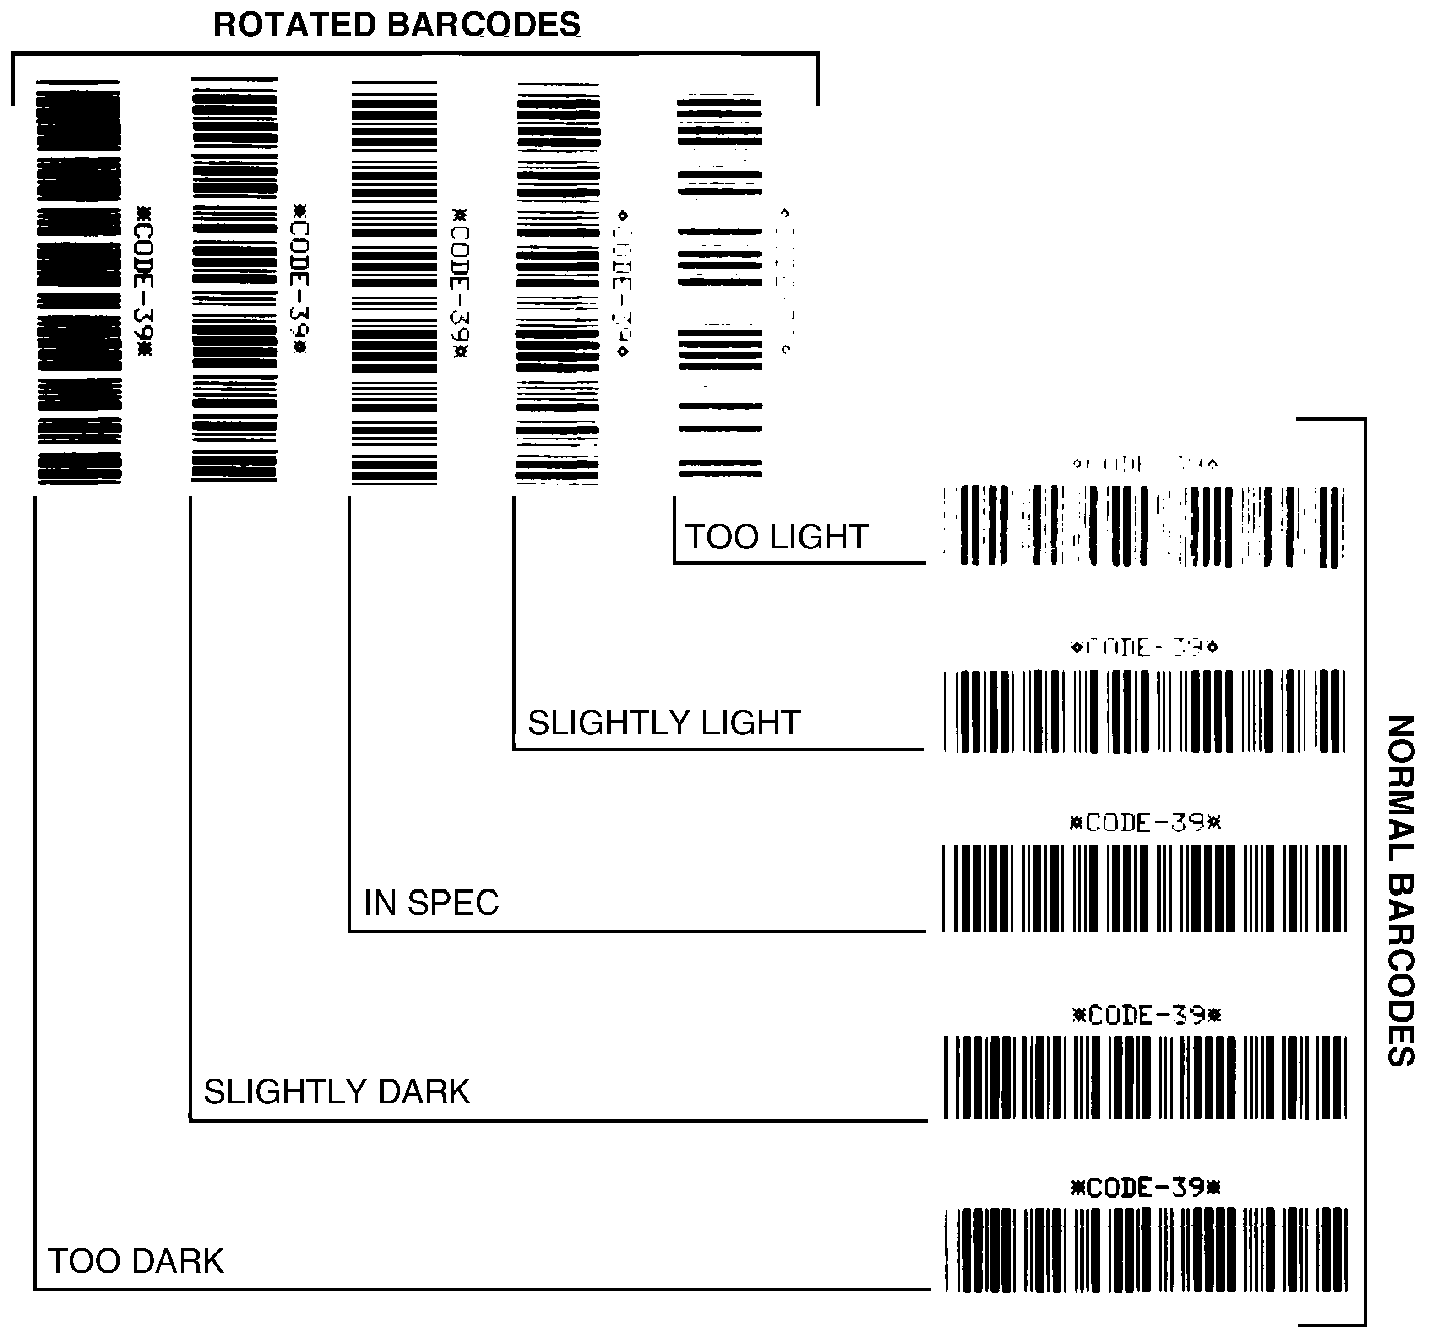
\includegraphics[width=0.82\textwidth]{figuras/zebra_darkness_comparison.png}

\vspace{2pt}
{\footnotesize Fonte: \citeonline{zebra_maintenance}.}
\end{figure}

A nota de uma varredura é a \textbf{menor} entre os parâmetros; a nota do símbolo
é a \textbf{média de dez varreduras} distribuídas ao longo da altura. Para 2D, a
ISO/IEC 15415 cumpre papel equivalente com parâmetros adaptados à matriz
\cite{iso15415}, e a marcação direta de peça (DPM) é tratada pela ISO/IEC 29158
\cite{iso29158}.

\noindent\textbf{Ponto metodológico importante.} A verificação \textit{conformante}
exige condições ópticas controladas --- fonte de luz definida, abertura de
medição, geometria e calibração de refletância --- providas por verificadores
certificados \cite{iso15426}. Uma imagem de câmera comum não reproduz essas
condições. Por isso, neste trabalho os parâmetros da norma são usados como
referencial conceitual e como indicadores aproximados, não como grau oficial ---
o que delimita honestamente o escopo (Seção~\ref{sec-fund}).

\subsection{Defeitos típicos de impressão térmica e suas causas}\label{sec-defeitos}

Impressoras térmicas de transferência (como a Zebra ZT411/ZT421) formam a imagem
aquecendo seletivamente uma cabeça de impressão que transfere tinta do
\textit{ribbon} para a mídia, prensada pelo rolete (\textit{platen}). Cada
componente falha de um modo com assinatura visual característica. A partir do guia
do usuário da ZT411/ZT421, do procedimento de manutenção e da base de
conhecimento da Zebra \cite{zebra_printquality}, consolida-se o mapeamento da
Tabela~\ref{tab-defeitos} --- que é, em si, uma das contribuições do trabalho.

\begin{table}[htb]
\centering
\caption{Mapeamento entre aparência do defeito, causa provável e ação corretiva}
\label{tab-defeitos}
\begin{tabular}{@{}p{4.4cm}p{4.2cm}p{4.6cm}@{}}
\toprule
\textbf{Defeito (aparência)} & \textbf{Causa provável} & \textbf{Ação corretiva típica}\\
\midrule
Código não escaneia; imagem ``suja'' & \textit{Darkness} alto demais ou pressão da
cabeça incorreta & Reduzir o \textit{darkness}; reduzir velocidade; ajustar pressão\\
Impressão clara (\textit{faded}) em toda a etiqueta & \textit{Darkness} baixo,
mídia/\textit{ribbon} incompatível ou alta velocidade & Elevar \textit{darkness};
trocar para combinação mídia-\textit{ribbon} adequada\\
Impressão clara/escura em um lado da etiqueta & Pressão \textbf{desigual} da cabeça
& Ajustar a pressão da cabeça (\textit{toggles})\\
Linhas cinza finas e angulares em etiquetas em branco & \textit{Ribbon} enrugado &
Corrigir tensão/alinhamento do \textit{ribbon}\\
Trilhas longas de impressão faltando & Elemento da cabeça danificado (linhas
brancas verticais) & Acionar assistência técnica (troca de cabeça)\\
\textit{Voids} no código; qualidade inconsistente & Cabeça de impressão \textbf{suja}
& Limpar cabeça e rolete com álcool isopropílico 99,7\%\\
Manchas (\textit{smudge}) & Mídia/\textit{ribbon} inadequados para alta velocidade
& Trocar por insumos recomendados\\
Perda de registro / deslocamento vertical & Rolete sujo, mídia mal carregada,
sensor descalibrado & Limpar rolete; recarregar mídia; calibrar sensores\\
\bottomrule
\end{tabular}

\vspace{2pt}
{\footnotesize Fonte: elaboração própria (2026), a partir de \citeonline{zebra_printquality}.}
\end{table}

A Figura~\ref{fig-defeitos-zebra} exemplifica, em etiquetas impressas reais, as
assinaturas visuais de vários desses defeitos, tal como documentadas pela Zebra
\cite{zebra_kb_printquality}. Note-se a correspondência com as classes reproduzidas
sinteticamente na Seção~\ref{sec-dados}.

\begin{figure}[htb]
\centering
\caption{Assinaturas visuais reais de defeitos de impressão térmica em etiquetas de códigos de barras}
\label{fig-defeitos-zebra}

\begin{minipage}[t]{0.31\textwidth}\centering
  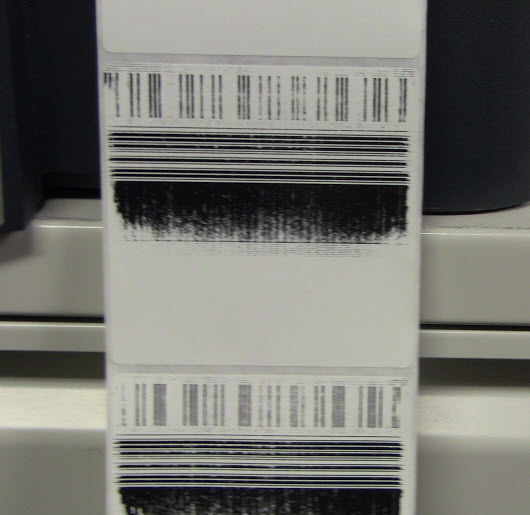
\includegraphics[width=\linewidth,height=3cm,keepaspectratio]{figuras/zebra_impressao_clara.jpg}\\[2pt]
  {\footnotesize (a) Impressão clara (\textit{faded})}
\end{minipage}\hfill
\begin{minipage}[t]{0.31\textwidth}\centering
  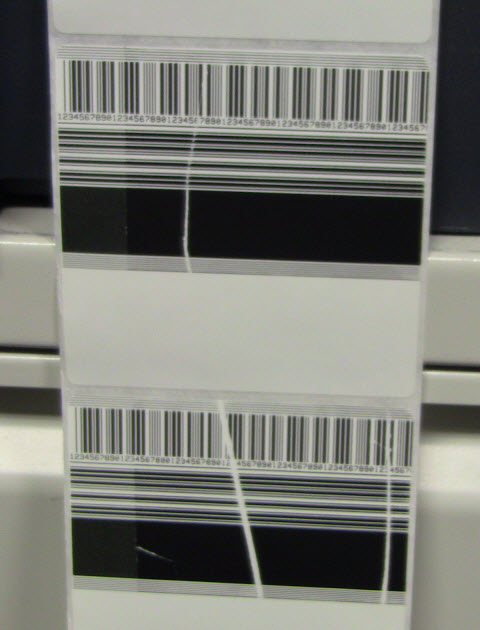
\includegraphics[width=\linewidth,height=3cm,keepaspectratio]{figuras/zebra_ribbon_enrugado.jpg}\\[2pt]
  {\footnotesize (b) \textit{Ribbon} enrugado}
\end{minipage}\hfill
\begin{minipage}[t]{0.31\textwidth}\centering
  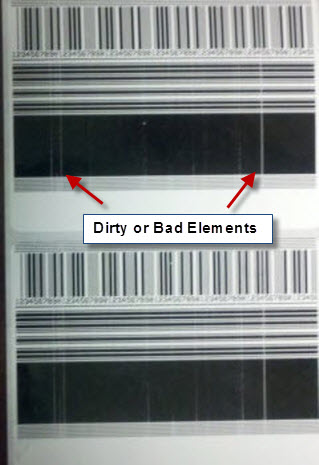
\includegraphics[width=\linewidth,height=3cm,keepaspectratio]{figuras/zebra_elemento_danificado.jpg}\\[2pt]
  {\footnotesize (c) Elemento da cabeça danificado}
\end{minipage}

\vspace{8pt}

\begin{minipage}[t]{0.31\textwidth}\centering
  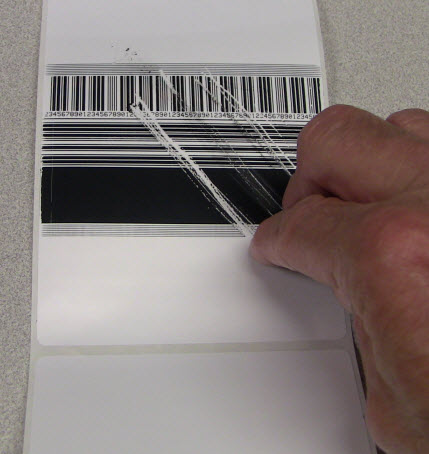
\includegraphics[width=\linewidth,height=3cm,keepaspectratio]{figuras/zebra_mancha.jpg}\\[2pt]
  {\footnotesize (d) Mancha (\textit{smear})}
\end{minipage}\hfill
\begin{minipage}[t]{0.31\textwidth}\centering
  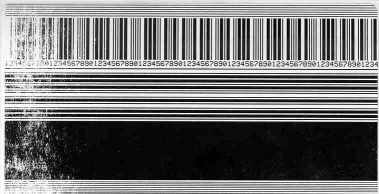
\includegraphics[width=\linewidth,height=3cm,keepaspectratio]{figuras/zebra_pressao_desigual.jpg}\\[2pt]
  {\footnotesize (e) Pressão desigual da cabeça}
\end{minipage}\hfill
\begin{minipage}[t]{0.31\textwidth}\centering
  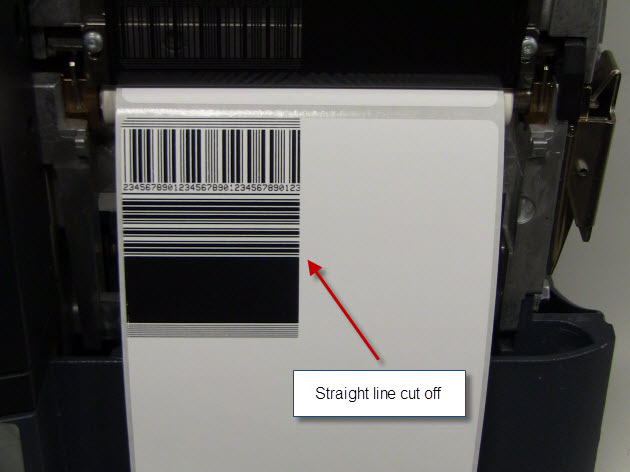
\includegraphics[width=\linewidth,height=3cm,keepaspectratio]{figuras/zebra_perda_registro.jpg}\\[2pt]
  {\footnotesize (f) Perda de registro (\textit{cutoff})}
\end{minipage}

\vspace{6pt}
{\footnotesize Fonte: \citeonline{zebra_kb_printquality}.}
\end{figure}

A manutenção preventiva atua sobre as causas de origem: a limpeza periódica da
cabeça e do rolete com álcool isopropílico 99,7\% (ou kit de manutenção Zebra) é
indicada quando surgem \textit{voids}, e a documentação alerta que
\textit{darkness} excessivo desgasta a cabeça prematuramente e pode ``queimar'' o
\textit{ribbon} \cite{zebra_printquality}. Esse conhecimento é o que alimenta o
agente de diagnóstico proposto na Seção~\ref{sec-proposta}.

\subsection{Processamento de imagens e visão computacional para inspeção}

O reconhecimento dos defeitos acima é um problema de \textbf{inspeção visual
automatizada}. As etapas clássicas envolvem:
\begin{alineas}
	\item \textbf{pré-processamento} --- conversão de cor, correção de iluminação
	e realce de contraste para atenuar variações de captura \cite{gonzalez2018};
	\item \textbf{localização/segmentação do símbolo} --- isolar a região do
	código na etiqueta, condição para medir refletância e detectar defeitos
	localizados \cite{szeliski2022};
	\item \textbf{detecção de objetos/defeitos} --- localizar e classificar
	regiões defeituosas; abordagens supervisionadas de um estágio (por exemplo, da
	família YOLO) são amplamente usadas em inspeção industrial;
	\item \textbf{classificação por redes convolucionais (CNN)} --- atribuir a
	classe de defeito a partir de características aprendidas, dispensando extração
	manual de atributos; e
	\item \textbf{detecção de anomalias} --- quando amostras de defeito real são
	escassas, métodos não supervisionados aprendem o ``normal'' e sinalizam
	desvios, contornando o desbalanceamento de dados.
\end{alineas}

A literatura recente de inspeção industrial converge nesses pilares e destaca um
desafio recorrente diretamente relevante a este trabalho: a \textbf{escassez de
imagens de defeito real}, que motiva aumento de dados e abordagens semi/não
supervisionadas \cite{frontiers2025anomaly,survey2022unsupervised}.

\subsection{Sistemas multiagentes e o \textit{Agent Development Kit} (ADK)}

Um \textbf{sistema multiagente} é um conjunto de agentes autônomos que colaboram
para uma meta comum, cada um responsável por uma subtarefa. O \textit{Agent
Development Kit} (ADK), apresentado pelo Google no Cloud NEXT 2025, é um
\textit{framework} de código aberto para construir e orquestrar esses sistemas
\cite{google_adk_blog}. Ele organiza os agentes em três tipos:
\begin{alineas}
	\item \textbf{agentes LLM} --- o ``raciocínio'', que interpreta entradas e
	decide ações;
	\item \textbf{agentes de \textit{workflow}} --- orquestradores de fluxo
	(sequencial, paralelo, em laço); e
	\item \textbf{agentes customizados} --- especialistas que encapsulam lógica ou
	modelos próprios (por exemplo, um modelo de visão).
\end{alineas}

Os agentes se organizam em uma \textbf{hierarquia} e se comunicam por estado
compartilhado, delegação e invocação explícita \cite{adk_docs}. A justificativa
central do paradigma --- e o argumento que este trabalho pretende testar
empiricamente --- é que decompor um problema em agentes especializados tende a ser
mais confiável, modular e manutenível do que um único modelo/prompt monolítico,
porque cada agente resolve uma tarefa mais simples e bem delimitada.

% ---------------------------------------------------------------------------
\section{Trabalhos relacionados}\label{sec-relacionados}
% ---------------------------------------------------------------------------

\subsection{Verificação normativa e diagnóstico de defeitos}

A base da verificação de qualidade são as normas ISO/IEC 15416 e 15415,
implementadas por verificadores comerciais que reportam notas A--F
\cite{iso15416,iso15415}. Há também soluções que inferem falhas do mecanismo de
impressão a partir da própria leitura --- por exemplo, detectando linhas não
impressas para gerar um relatório de manutenção do cabeçote e alertar antes da
falha total \cite{patent9826106}. \textbf{Limitação comum:} dependem de
\textit{hardware} dedicado e/ou entregam a nota/alerta, sem um diagnóstico de
causa-raiz acionável e contextualizado pela documentação do fabricante.

\subsection{Inspeção visual de defeitos com aprendizado profundo}

A inspeção industrial baseada em aprendizado profundo é sistematizada em
levantamentos recentes que cobrem CNNs, detecção de objetos e detecção de
anomalias, com ênfase no problema de dados escassos
\cite{frontiers2025anomaly,survey2022unsupervised}. Aplicações diretas ao domínio
de impressão incluem a detecção de defeitos em tecidos estampados com CNN
\cite{fabric2021cnn} e a detecção/localização de anomalias em manufatura aditiva
por transferência de aprendizado \cite{fff2024thermal}. \textbf{Limitação comum:}
focam a classificação/localização do defeito visual, sem ligá-lo à causa física
do processo nem a uma ação corretiva.

\subsection{Sistemas multiagentes aplicados a tarefas de visão}

A orquestração multiagente com ADK e \textit{frameworks} correlatos vem sendo
aplicada a tarefas complexas que se beneficiam de decomposição, tratando agentes
especializados como ferramentas de um agente raiz \cite{google_adk_blog}.
\textbf{Lacuna observada:} a combinação de orquestração multiagente com inspeção
de qualidade de impressão de códigos de barras --- em especial acoplando detecção
visual a diagnóstico fundamentado em documentação técnica --- é pouco explorada.

\subsection{Lacuna que este trabalho preenche}

Reunindo os três eixos: os verificadores dão nota mas não causa; os métodos de
visão detectam o defeito mas não a causa nem a correção; e a orquestração
multiagente é madura porém raramente aplicada a este domínio. Este trabalho se
posiciona nessa interseção, propondo um sistema de baixo custo, servido por API,
que combina estimativa de indicadores de qualidade, detecção visual de defeitos
físicos e diagnóstico de causa-raiz fundamentado na documentação da Zebra,
orquestrados por agentes especializados. O Quadro comparativo da
Tabela~\ref{tab-comparativo} posiciona este trabalho frente às abordagens
existentes.

\begin{table}[htb]
\centering
\caption{Comparativo entre abordagens quanto aos recursos oferecidos}
\label{tab-comparativo}
\begin{tabular}{@{}p{4.2cm}*{4}{>{\centering\arraybackslash}p{2.2cm}}@{}}
\toprule
\textbf{Abordagem} & \textbf{Nota ISO} & \textbf{Defeito físico} &
\textbf{Causa-raiz} & \textbf{Sem \textit{hardware} dedicado}\\
\midrule
Verificadores certificados & Sim & Não & Não & Não\\
Visão computacional (CNN/anomalia) & Não & Sim & Não & Sim\\
Detecção via leitura (patente) & Parcial & Parcial & Parcial & Não\\
\textbf{Este trabalho} & Aprox. & Sim & Sim & Sim\\
\bottomrule
\end{tabular}

\vspace{2pt}
{\footnotesize Fonte: elaboração própria (2026).}
\end{table}

% ---------------------------------------------------------------------------
\section{Metodologia}\label{sec-metodo}
% ---------------------------------------------------------------------------

\subsection{Tipo de pesquisa}

Pesquisa de natureza \textbf{aplicada}, abordagem \textbf{quantitativa} e objetivo
\textbf{exploratório-experimental}: constrói-se um artefato (o sistema) e mede-se
seu desempenho em condições controladas, com procedimento experimental.

\subsection{Conjunto de dados}\label{sec-dados}

O problema tem duas naturezas distintas --- a \textbf{legibilidade da captura} (a
imagem do código está boa o suficiente para ler?) e o \textbf{defeito de
impressão} (que falha do processo produziu a marca?) --- e cada uma exige um tipo
de dado. Por isso, adota-se uma estratégia de \textbf{duas trilhas}.

\noindent\textbf{Trilha A --- imagens reais de captura (base disponível).}
Conjunto de 52 imagens reais de códigos de barras fotografados em produtos e
embalagens, em tons de cinza, sob ângulo, reflexo, curvatura e fundos variados, já
organizadas por simbologia, conforme a Tabela~\ref{tab-trilhaA}. Esse conjunto é
usado para treinar/avaliar o agente de leitura/decodificação e o agente de
indicadores de legibilidade. Como são todas 1D, as amostras 2D são complementadas
na Trilha B.

\begin{table}[htb]
\centering
\caption{Trilha A --- imagens reais por simbologia}
\label{tab-trilhaA}
\begin{tabular}{@{}lc@{}}
\toprule
\textbf{Simbologia} & \textbf{N.º de imagens}\\
\midrule
EAN-13 & 19\\
Code 39 & 6\\
Code 128 & 5\\
EAN-8 & 5\\
\textit{Interleaved 2 of 5} & 5\\
EAN-13 (\textit{add-on} 2) & 4\\
EAN-13 (\textit{add-on} 5) & 4\\
Pharmacode & 4\\
\midrule
\textbf{Total} & \textbf{52}\\
\bottomrule
\end{tabular}

\vspace{2pt}
{\footnotesize Fonte: elaboração própria (2026).}
\end{table}

\noindent\textbf{Trilha B --- defeitos de impressão sintéticos (gerados).} Para
treinar o agente de defeitos físicos não há um conjunto público rotulado de
defeitos de impressão térmica, e as fotos da base de conhecimento da Zebra são
material protegido por direitos autorais. Adota-se, então, \textbf{geração
sintética controlada}: a partir de códigos limpos (1D e 2D), aplicam-se
transformações que reproduzem a assinatura visual de cada defeito descrito na
documentação Zebra \cite{zebra_printquality}, conforme a Tabela~\ref{tab-trilhaB}.
Um gerador de referência foi implementado (\texttt{gerar\_dataset.py}) e produz as
sete classes de forma balanceada, com divisão automática em treino/validação/teste
(70/15/15) e parâmetros de defeito amostrados aleatoriamente em faixas definidas.
A Figura~\ref{fig-dataset} ilustra amostras das classes geradas.

\begin{table}[htb]
\centering
\caption{Trilha B --- classes de defeito e transformação sintética correspondente}
\label{tab-trilhaB}
\begin{tabular}{@{}p{4.6cm}p{5.0cm}p{4.0cm}@{}}
\toprule
\textbf{Classe de defeito} & \textbf{Transformação sintética} & \textbf{Sintoma reproduzido}\\
\midrule
Cabeça queimada (elemento danificado) & Linhas brancas verticais contínuas &
Trilhas longas de impressão faltando\\
\textit{Ribbon} enrugado & Faixas claras finas e diagonais & Linhas cinza angulares\\
Ponto queimado / \textit{darkness} alto & Manchas escuras localizadas &
Excesso de temperatura\\
Impressão clara (\textit{darkness} baixo) & Redução de contraste global &
\textit{Faded} / mídia-\textit{ribbon} incompatível\\
Pressão desigual & Borrão direcional (gradiente em um lado) & Densidade não uniforme\\
Cabeça suja (\textit{voids}) & Falhas brancas pontuais nas barras & \textit{Voids} no código\\
Sem defeito & (código limpo) & Classe de controle\\
\bottomrule
\end{tabular}

\vspace{2pt}
{\footnotesize Fonte: elaboração própria (2026).}
\end{table}

\begin{figure}[htb]
\centering
\caption{Amostras do conjunto sintético de defeitos, uma classe por bloco}
\label{fig-dataset}
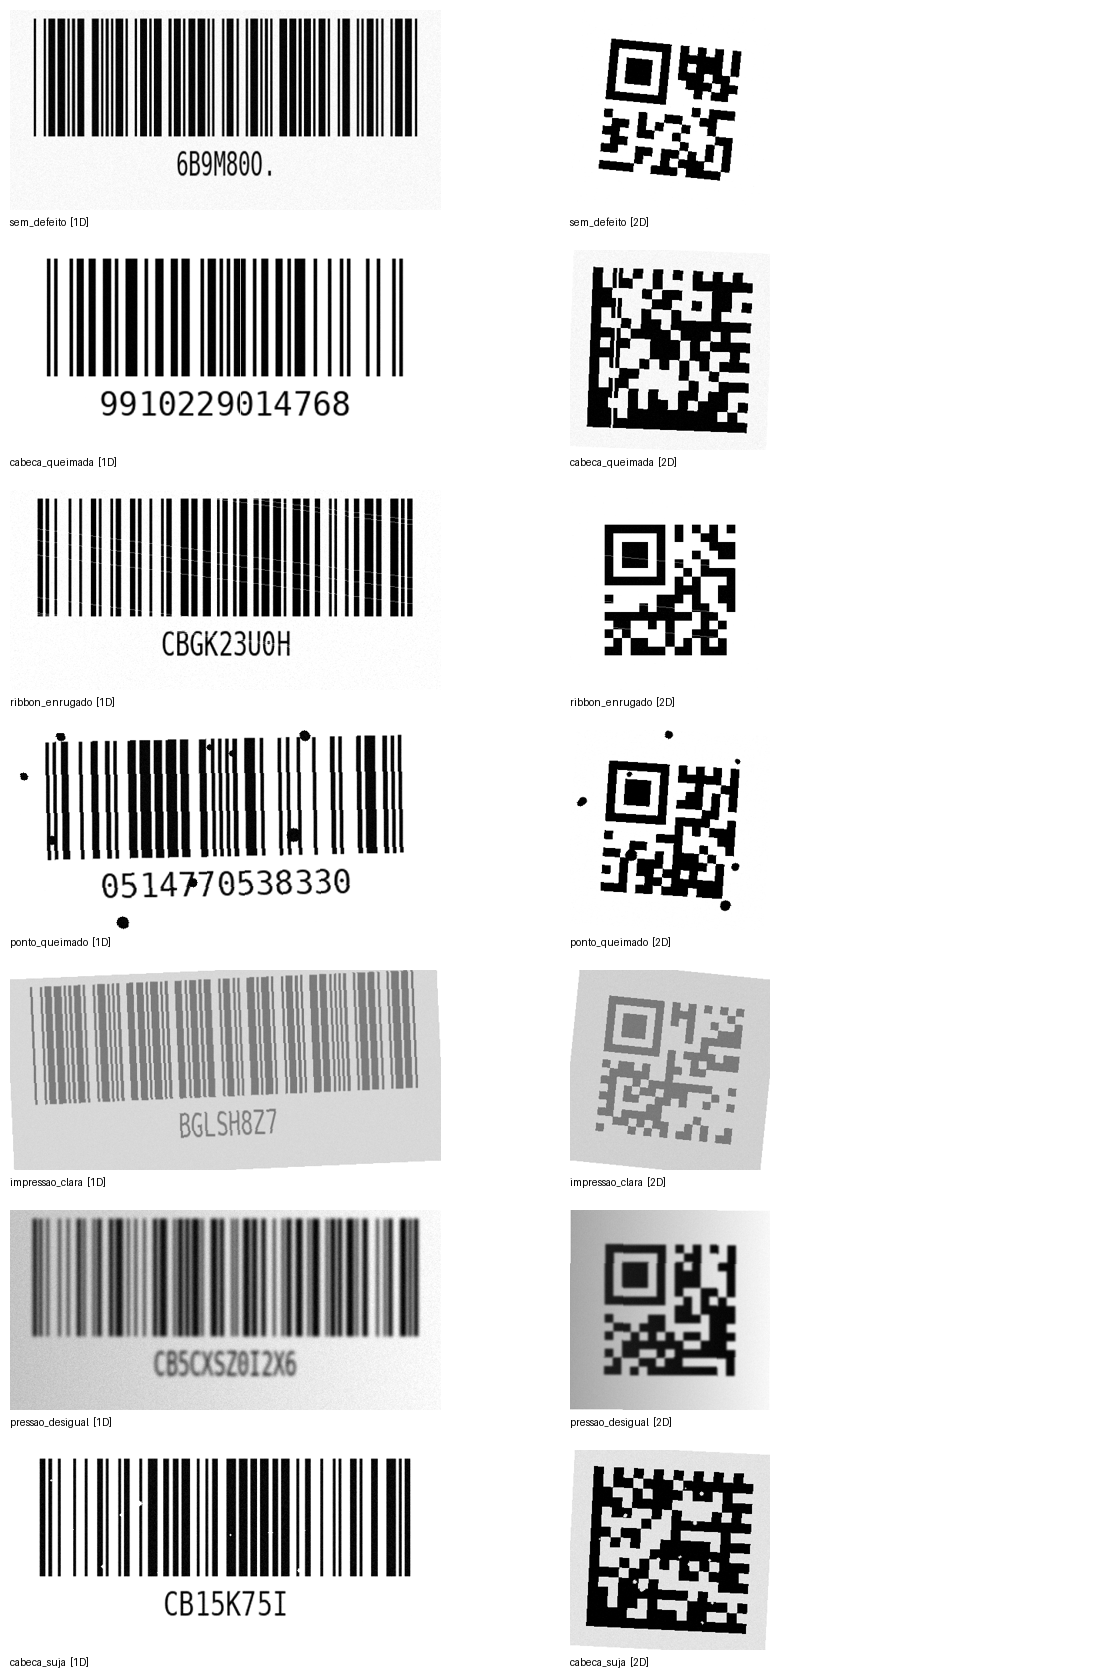
\includegraphics[width=0.95\textwidth]{figuras/dataset_preview.png}

\vspace{2pt}
{\footnotesize Fonte: elaboração própria (2026), gerada por \texttt{gerar\_dataset.py}.}
\end{figure}

Essa abordagem é reprodutível, balanceável e livre de restrições autorais, e é
prática consolidada na literatura de inspeção quando amostras reais são escassas
\cite{frontiers2025anomaly,survey2022unsupervised}.

\noindent\textbf{Divisão e aumento de dados.} Cada trilha é dividida em
treino/validação/teste (70/15/15), estratificando por classe. Sobre a Trilha A
aplica-se aumento de dados clássico (rotação, variação de brilho/contraste,
recortes) para ampliar a variabilidade de captura. Os parâmetros dos defeitos
sintéticos (intensidade, quantidade, posição) são amostrados aleatoriamente em
faixas definidas, para evitar que o modelo aprenda um padrão fixo.

\noindent\textbf{Datasets externos (complementares).} Para avaliar a generalização
para imagens reais e ampliar a variabilidade, o conjunto pode ser complementado por
bases públicas de defeitos de códigos de barras e etiquetas disponíveis no
\textit{Roboflow Universe}\footnote{Busca por conjuntos de dados de defeitos:
\url{https://universe.roboflow.com/search?q=barcode+damage}; termos correlatos:
\textit{barcode defect} e \textit{label print quality}.} --- empregadas
preferencialmente como conjunto de teste de generalização (sintético $\rightarrow$
real). O projeto inclui um utilitário de \textit{download}
(\texttt{baixar\_roboflow.py}) para essa finalidade.

\subsection{Ferramentas utilizadas}

\begin{alineas}
	\item \textbf{visão computacional:} Python, OpenCV e \textbf{PyTorch}. O
	PyTorch é hoje o \textit{framework} predominante na comunidade acadêmica, o
	que favorece a reprodutibilidade e a comparação com trabalhos correlatos. Para
	atender a máquinas modestas, adota-se transferência de aprendizado com um
	\textit{backbone} leve (\textbf{MobileNetV3-Small} ou \textbf{EfficientNet-B0}),
	que treina bem em GPU de entrada ou mesmo CPU; como a inferência é servida pela
	API (lado servidor), o dispositivo do usuário não precisa executar o modelo;
	\item \textbf{decodificação e OCR:} \texttt{pyzbar} (ZBar) para decodificar o
	símbolo e verificar a legibilidade, e o \textbf{Tesseract} (\texttt{pytesseract})
	para o reconhecimento óptico do texto humano-legível impresso junto às barras;
	\item \textbf{orquestração multiagente:} \textit{Agent Development Kit} (ADK)
	\cite{google_adk_blog}, com \textbf{Gemini} como modelo LLM dos agentes de
	raciocínio, aproveitando a integração nativa do ADK com o ecossistema Google;
	\item \textbf{entrega:} API única (FastAPI) que serve um \textbf{chat} web
	internacionalizado (português/inglês) para o envio da imagem e que pode,
	também, alimentar um aplicativo Android; e
	\item \textbf{escrita e gestão bibliográfica:} \LaTeX{} (abnTeX2/Overleaf) e
	Zotero.
\end{alineas}

As técnicas empregadas correspondem diretamente ao conteúdo da disciplina de Visão
Computacional em que este trabalho se insere --- aquisição e representação de imagens
com OpenCV; limiarização e filtragem; detecção de arestas e contornos; segmentação;
morfologia matemática; descritores e características; classificadores; e redes neurais
convolucionais. O projeto, assim, exercita de ponta a ponta o pipeline clássico de
visão computacional, culminando em uma CNN para a classificação dos defeitos.

\subsection{Ambiente experimental}

Os experimentos foram executados em \textbf{CPU} (Intel Core i7-1185G7, 8
\textit{threads}, 31\,GB de RAM), \textbf{sem GPU dedicada}, com Python 3.12, PyTorch
2.13 (CPU), \textit{torchvision} 0.28 e OpenCV 4.10; o ambiente Python é gerenciado com
\texttt{uv}. O \textit{fine-tuning} da CNN sobre o conjunto sintético levou poucos
minutos nessa configuração, evidenciando a viabilidade em máquinas modestas.
\textit{Observação:} como o contraste medido depende fortemente da captura, padronizar
iluminação e distância é parte do rigor experimental para as imagens reais.

\subsection{Métricas de avaliação}

\begin{alineas}
	\item \textbf{classificação de defeitos:} acurácia, precisão, revocação e F1
	por classe, além da matriz de confusão;
	\item \textbf{detecção/localização (se houver):} mAP e IoU;
	\item \textbf{indicadores de qualidade:} concordância entre o indicador
	estimado e a referência disponível (verificador, se houver, ou rótulo
	especialista); e
	\item \textbf{benefício do multiagente:} comparação das métricas acima entre a
	arquitetura multiagente e a abordagem monolítica (Seção~\ref{sec-baseline}),
	além de latência e interpretabilidade do laudo.
\end{alineas}

% ---------------------------------------------------------------------------
\section{Proposta da solução}\label{sec-proposta}
% ---------------------------------------------------------------------------

\subsection{Arquitetura da solução}

A solução adota o padrão \textbf{hierárquico} do ADK \cite{adk_docs}, no qual um
agente raiz coordena agentes especializados. A tarefa ``avaliar uma etiqueta'' é
decomposta em quatro análises especializadas e uma etapa de síntese, explorando
dois recursos de orquestração do ADK: execução paralela para as análises
independentes e execução sequencial para as etapas que dependem das anteriores. O
sistema é composto por:
\begin{alineas}
	\item \textbf{agente de leitura/decodificação} --- com OpenCV, segmenta a região
	do código (gradiente, limiarização e morfologia); decodifica com o \texttt{pyzbar}
	(simbologia e conteúdo) e lê o texto humano-legível com o Tesseract (OCR); retorna
	legível/ilegível e o conteúdo;
	\item \textbf{agente de indicadores de qualidade} --- sobre a região segmentada
	pelo OpenCV, estima indicadores inspirados na ISO/IEC 15416 (contraste,
	uniformidade e nitidez), sempre como aproximação (Seção~\ref{sec-qualidade});
	\item \textbf{agente de defeitos físicos} --- classifica o defeito de impressão
	(as sete classes da Seção~\ref{sec-dados}) usando a CNN treinada, exposta ao
	ADK como ferramenta;
	\item \textbf{agente de diagnóstico} --- agente LLM (Gemini) que, com os
	resultados anteriores e uma ferramenta de recuperação sobre a documentação
	Zebra (RAG), infere a causa provável e a ação corretiva; e
	\item \textbf{agente de laudo} --- consolida tudo em um JSON estruturado
	devolvido pela API.
\end{alineas}

Os agentes 1--3 são independentes e rodam em paralelo (\texttt{ParallelAgent}); o
agente 4 depende das saídas dos três e o agente 5 depende do 4, formando uma
cadeia (\texttt{SequentialAgent}). A comunicação entre agentes usa o estado
compartilhado da sessão: cada agente grava seu resultado em uma chave
(\texttt{output\_key}) e os seguintes leem essas chaves.

% >>> Inserir aqui a figura da arquitetura (árvore de agentes). Coloque o
% arquivo em figuras/arquitetura.png e descomente o bloco abaixo.
% \begin{figure}[htb]
% \centering
% \caption{Arquitetura multiagente da solução (árvore de agentes).}
% \label{fig-arquitetura}
% \includegraphics[width=0.8\textwidth]{figuras/arquitetura.png}
% \vspace{2pt}
% {\footnotesize Fonte: elaboração própria (2026).}
% \end{figure}

\subsection{Fluxograma do processamento}

O fluxo ponta a ponta é: envio da imagem no chat $\rightarrow$ \texttt{POST /analisar}
na API $\rightarrow$ pré-processamento e segmentação com OpenCV $\rightarrow$
\textbf{verificação da presença} de um código de barras $\rightarrow$ (havendo código)
\texttt{ParallelAgent} executa, em paralelo, a leitura/decodificação (\texttt{pyzbar}
$+$ OCR Tesseract), os indicadores de qualidade e a classificação do defeito (CNN)
$\rightarrow$ o agente de diagnóstico consome as três saídas e consulta a
documentação Zebra $\rightarrow$ o agente de laudo agrega em JSON $\rightarrow$
resposta única $\rightarrow$ renderização no chat.

\noindent\textbf{Decisão de projeto: curto-circuito de presença do código.} A
verificação da presença do código de barras ocorre \textbf{antes} da inspeção
pesada. Se nenhum código é detectado na imagem, o sistema retorna um laudo
\textbf{mínimo} --- apenas o aviso ``Nenhum código de barras detectado na
imagem.'' ---, sem executar a CNN de classificação nem invocar o agente LLM. A
motivação é dupla: (i) \textbf{evitar diagnósticos espúrios}, isto é, não
apresentar ao operador uma causa/correção plausível para uma imagem que sequer
contém um código (falsa sensação de resultado útil); e (ii) \textbf{economizar
processamento e chamadas de API} ao Gemini, que só são disparados quando há, de
fato, o que inspecionar. A legibilidade bem-sucedida já implica presença; caso
contrário, um detector leve sobre a imagem em tons de cinza decide o
curto-circuito.

% >>> Inserir aqui o fluxograma (bloco paralelo + cadeia sequencial) em
% figuras/fluxograma.png e descomentar bloco análogo ao anterior.

\subsection{Algoritmos empregados}

\begin{alineas}
	\item \textbf{segmentação do símbolo:} localização da região do código e das
	zonas de silêncio (limiarização adaptativa mais operações morfológicas, ou um
	detector leve treinado);
	\item \textbf{estimativa de indicadores:} a partir da imagem em tons de cinza,
	extração de perfis de refletância aproximados e cálculo de contraste e de
	medidas de uniformidade por elemento --- apresentados como indicadores, não
	como grau ISO oficial;
	\item \textbf{classificação de defeitos:} CNN com \textit{backbone} leve
	(MobileNetV3-Small ou EfficientNet-B0) e transferência de aprendizado, treinada
	no conjunto sintético da Seção~\ref{sec-dados} e testada na generalização para
	imagens reais; e
	\item \textbf{diagnóstico:} recuperação (RAG) sobre a base de conhecimento
	estruturada (Seção~\ref{sec-defeitos}) e raciocínio do agente LLM para ordenar
	as causas prováveis.
\end{alineas}

\subsection{Detalhes da implementação}

Cada especialista é definido como um agente do ADK; os modelos e rotinas de visão
computacional (OpenCV, \texttt{pyzbar}, Tesseract e a CNN em PyTorch) são expostos
como \textbf{ferramentas} (funções Python) que o ADK encapsula automaticamente. O
código é organizado no pacote \texttt{inspetor} (módulos \texttt{visao},
\texttt{rede}, \texttt{kb}, \texttt{diagnostico}, \texttt{ferramentas} e
\texttt{agentes}) e na camada \texttt{app} (CLI, API e chat web). O trecho da
Listagem~\ref{lst-agentes} é uma implementação de referência (a API do ADK evolui ---
consultar a documentação oficial \cite{adk_docs}).

\begin{lstlisting}[language=Python,caption={agentes.py --- implementação de referência (Google ADK + Gemini)},label=lst-agentes]
# agentes.py -- implementacao de referencia (Google ADK + Gemini)
from google.adk.agents import LlmAgent, ParallelAgent, SequentialAgent

MODEL = "gemini-flash-latest"

# ---- Ferramentas: rotinas de visao computacional (locais) ----
def decodificar_codigo(caminho_imagem: str) -> dict:
    """Localiza e decodifica o codigo. Retorna simbologia, conteudo e se e legivel."""
    from inspetor.visao import decodificar   # OpenCV + pyzbar
    return decodificar(caminho_imagem)        # {"legivel": bool, "simbologia": str, "conteudo": str}

def estimar_indicadores(caminho_imagem: str) -> dict:
    """Estima indicadores aproximados inspirados na ISO/IEC 15416 (nao e grau oficial)."""
    from inspetor.visao import indicadores
    return indicadores(caminho_imagem)        # {"contraste": float, "uniformidade": float}

def classificar_defeito(caminho_imagem: str) -> dict:
    """Classifica o defeito de impressao com a CNN treinada (7 classes)."""
    from inspetor.rede import prever           # checkpoint MobileNetV3-Small (PyTorch)
    return prever(caminho_imagem)             # {"classe": str, "confianca": float}

def buscar_documentacao_zebra(sintomas: str) -> str:
    """Recupera trechos relevantes da base de conhecimento estruturada (RAG)."""
    from inspetor.kb import buscar
    return buscar(sintomas)

# ---- Agentes especialistas (analises independentes -> paralelo) ----
agente_leitura = LlmAgent(
    name="leitura", model=MODEL, tools=[decodificar_codigo],
    instruction="Chame decodificar_codigo com a imagem e reporte se o codigo e legivel.",
    output_key="leitura",
)
agente_indicadores = LlmAgent(
    name="indicadores", model=MODEL, tools=[estimar_indicadores],
    instruction="Chame estimar_indicadores e reporte contraste e uniformidade.",
    output_key="indicadores",
)
agente_defeito = LlmAgent(
    name="defeito", model=MODEL, tools=[classificar_defeito],
    instruction="Chame classificar_defeito e reporte a classe e a confianca.",
    output_key="defeito",
)
analise_paralela = ParallelAgent(
    name="analise_paralela",
    sub_agents=[agente_leitura, agente_indicadores, agente_defeito],
)

# ---- Diagnostico (depende das analises) ----
agente_diagnostico = LlmAgent(
    name="diagnostico", model=MODEL, tools=[buscar_documentacao_zebra],
    instruction=(
        "Dado o defeito detectado ({defeito}), a legibilidade ({leitura}) e os "
        "indicadores ({indicadores}), use buscar_documentacao_zebra para fundamentar "
        "e proponha a CAUSA PROVAVEL e a ACAO CORRETIVA, citando o trecho de origem."
    ),
    output_key="diagnostico",
)

# ---- Laudo final (JSON estruturado) ----
agente_laudo = LlmAgent(
    name="laudo", model=MODEL,
    instruction=(
        "Consolide {leitura}, {indicadores}, {defeito} e {diagnostico} em um JSON com as "
        "chaves: legivel, simbologia, indicadores, defeito, causa_provavel, "
        "correcao_sugerida, confianca_geral. Responda SOMENTE o JSON."
    ),
    output_key="laudo",
)

# ---- Orquestrador raiz: paralelo -> diagnostico -> laudo ----
root_agent = SequentialAgent(
    name="inspetor_etiqueta",
    sub_agents=[analise_paralela, agente_diagnostico, agente_laudo],
)
\end{lstlisting}

A API expõe um \textbf{endpoint único} que devolve o laudo e serve a página de chat:
a mesma porta atende o chat web e pode atender um aplicativo Android
(Listagem~\ref{lst-api}). Além da imagem, o endpoint recebe do chat dois campos de
formulário --- o \texttt{idioma} do laudo (\texttt{pt-BR}/\texttt{en-US}) e o
\texttt{inspetor} (motor de diagnóstico) ---, que são repassados ao pipeline; a
página, por sua vez, recebe do servidor o nome do modelo LLM ativo, injetado na
resposta. Por robustez, a Listagem~\ref{lst-api} usa o \textbf{pipeline direto}
(\texttt{analisar\_imagem}), que funciona mesmo sem chave do Gemini; o grafo do ADK
(Listagem~\ref{lst-agentes}) é a variante orquestrada.

\begin{lstlisting}[language=Python,caption={api.py --- FastAPI (esboço)},label=lst-api]
# api.py -- FastAPI: serve o chat e o endpoint unico de analise
from fastapi import FastAPI, UploadFile, File, Form
from fastapi.responses import HTMLResponse, JSONResponse
from inspetor.ferramentas import analisar_imagem   # pipeline direto (robusto)

app = FastAPI()

@app.get("/")                                       # pagina de chat (envio da imagem)
def chat():
    pagina = open("app/chat.html", encoding="utf-8").read()
    return HTMLResponse(injetar_modelo_ativo(pagina))  # informa o LLM ativo a UI

@app.post("/analisar-htmx")                         # idioma + motor escolhidos na UI
async def analisar(imagem: UploadFile = File(...),
                   idioma: str = Form("pt-BR"),     # pt-BR | en-US (laudo bilingue)
                   inspetor: str = Form("llm")):    # llm | kb | auto
    caminho = await salvar_temp(imagem)             # persiste a imagem enviada
    usar_gemini = inspetor != "kb"                  # "kb" forca as regras Zebra
    laudo = analisar_imagem(caminho, usar_gemini=usar_gemini, idioma=idioma)
    return HTMLResponse(cartao_laudo_html(laudo, idioma))  # cartao do laudo (chat)
\end{lstlisting}

A Listagem~\ref{lst-laudo} mostra o esquema do laudo (resposta da API).

\begin{lstlisting}[language={},caption={Esquema do laudo devolvido pela API (JSON)},label=lst-laudo]
{
  "legivel": true,
  "codigo_detectado": true,
  "simbologia": "CODE128",
  "conteudo": "CB123",
  "texto_ocr": "CB123",
  "indicadores": { "contraste": 0.82, "uniformidade": 0.74, "nitidez": 0.60 },
  "defeito": { "classe": "ribbon_enrugado", "classe_pt": "Ribbon enrugado",
               "confianca": 0.91 },
  "causa_provavel": "Carregamento/tensao incorretos do ribbon (enrugamento)",
  "correcao_sugerida": "Verificar tensao, alinhamento e percurso do ribbon",
  "fonte": "Zebra Technologies (2024)",
  "via_diagnostico": "regras",
  "confianca_geral": 0.91
}
\end{lstlisting}

\subsection{Interface de uso: chat de inspeção}

A solução é entregue como um \textbf{chat}: o usuário envia a foto de uma etiqueta e
recebe, em resposta, um cartão de laudo estruturado. A mesma API atende uma página web
de chat e uma interface de linha de comando, e o grafo do ADK também pode ser exposto
pelo utilitário \texttt{adk web}. Por robustez, o sistema oferece dois caminhos com a
mesma saída: o \textbf{pipeline direto} (chamadas de função encadeadas, que funciona
mesmo sem chave do Gemini, recorrendo às regras da base de conhecimento Zebra) e o
\textbf{pipeline orquestrado} pelo ADK. O primeiro serve, ainda, de \textit{baseline}
monolítico na comparação da Seção~\ref{sec-baseline}. A Figura~\ref{fig-chat-inspetor}
mostra o sistema em funcionamento: a etiqueta enviada pelo usuário e o laudo devolvido,
com a leitura do código decodificado, os indicadores de qualidade, o defeito
classificado e a causa provável com a correção sugerida.

\begin{figure}[htb]
\centering
\caption{Inspetor de Etiquetas em execução no chat: etiqueta enviada e laudo completo (leitura, indicadores, defeito, causa e correção)}
\label{fig-chat-inspetor}
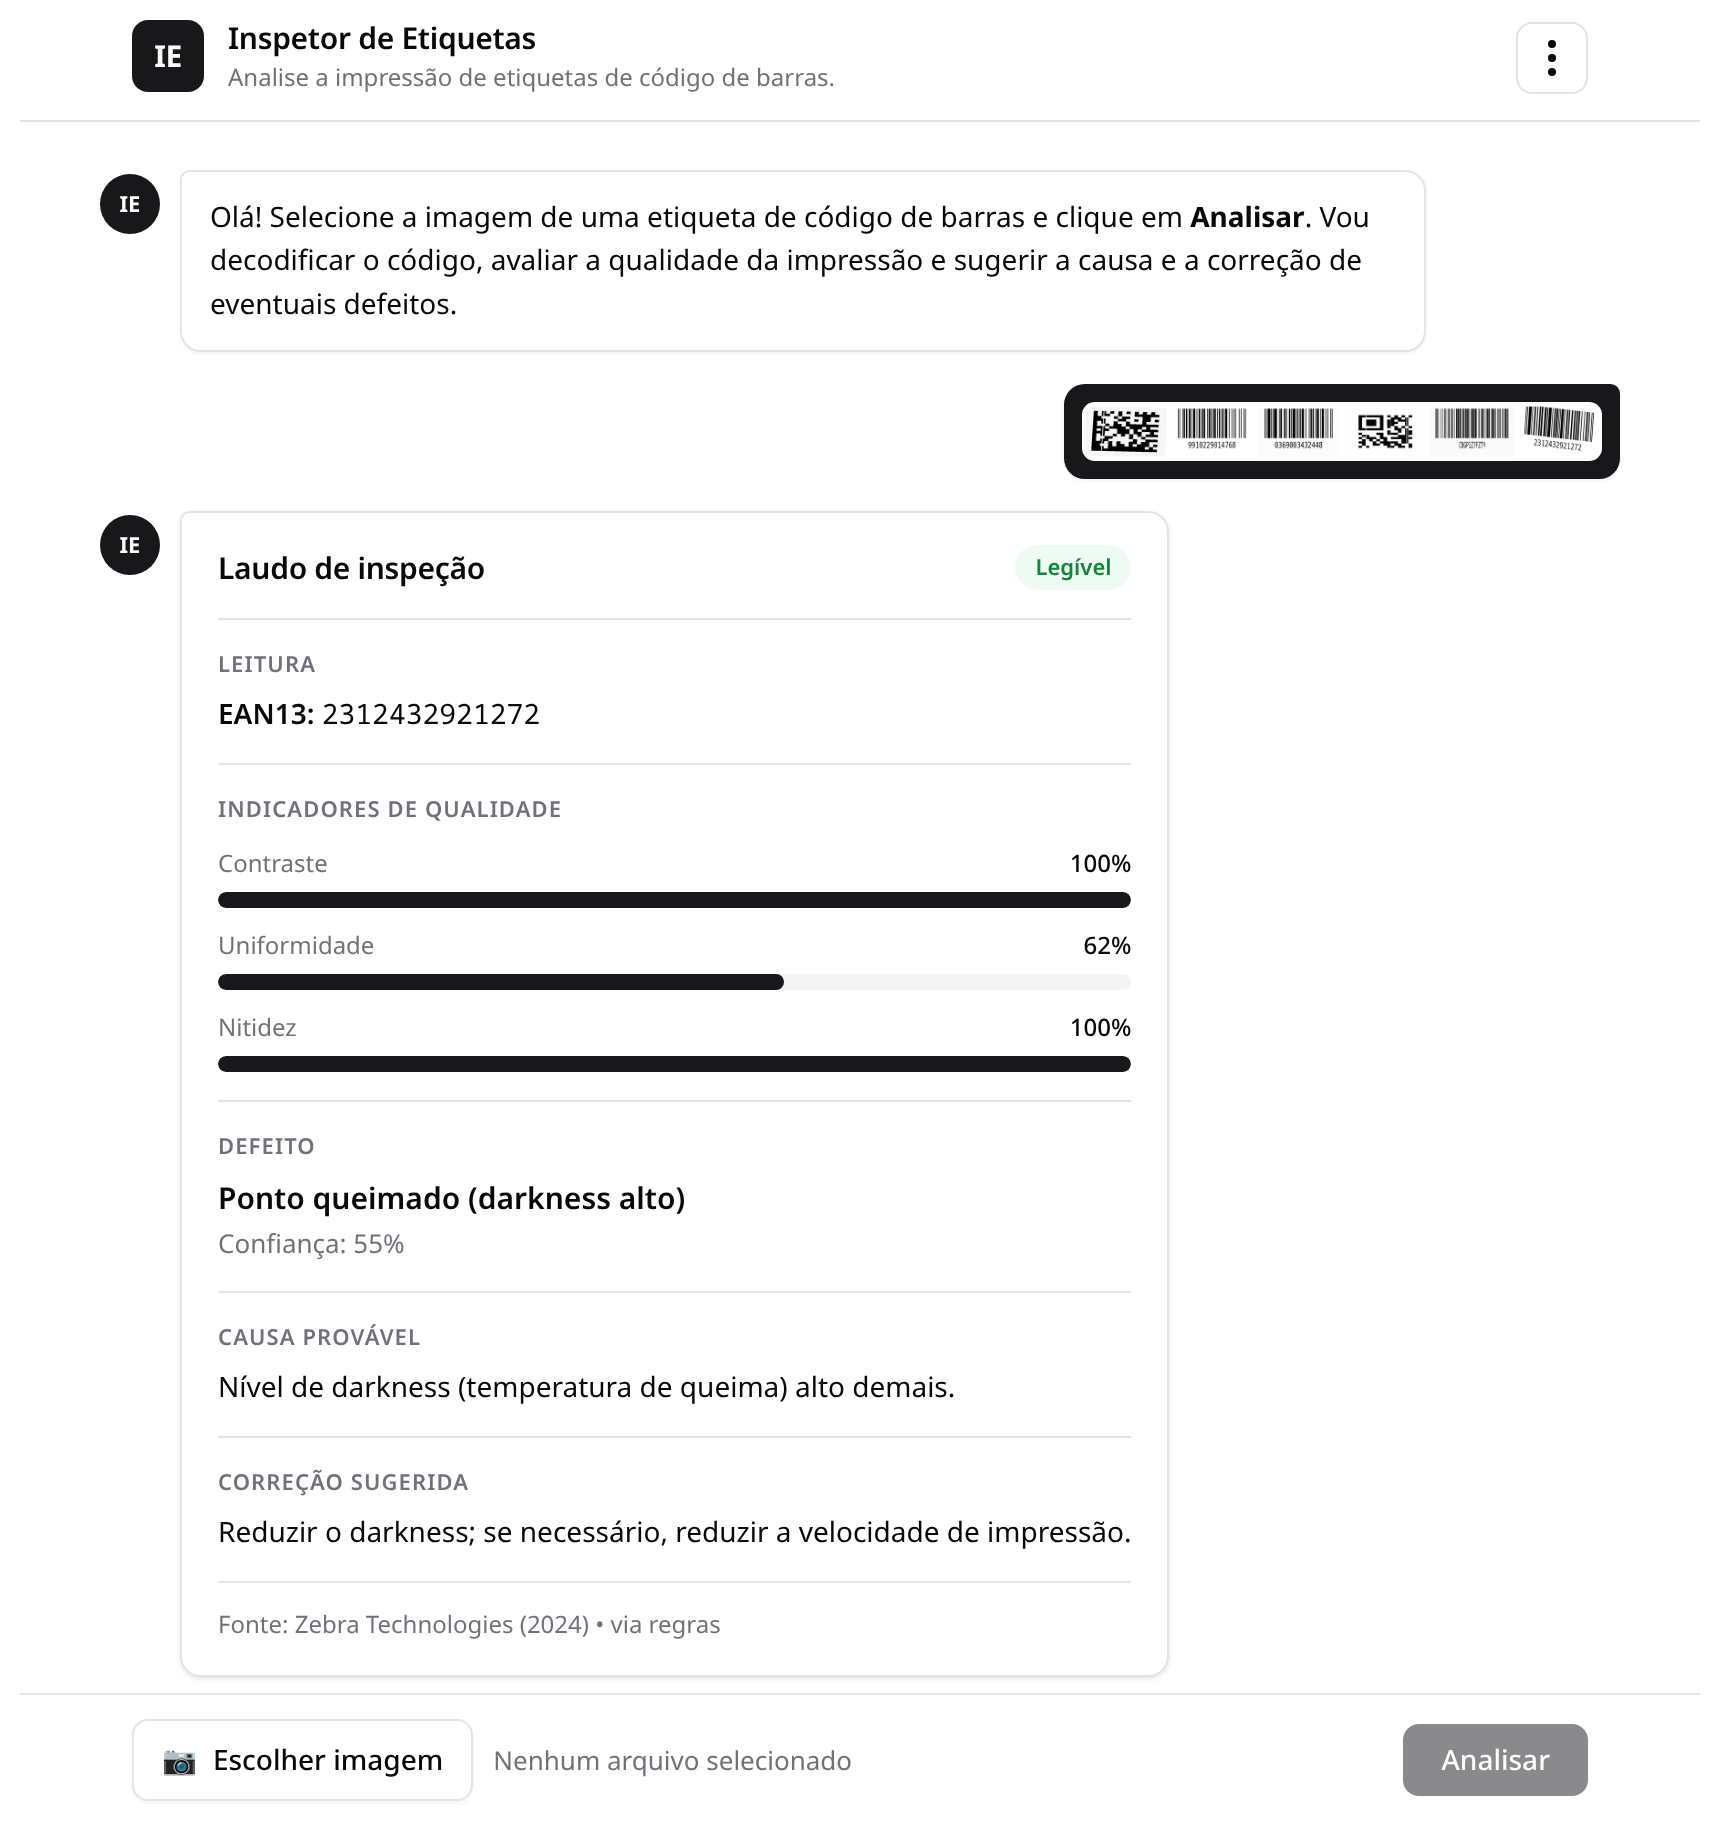
\includegraphics[width=0.62\textwidth]{figuras/chat_inspetor.png}

\vspace{2pt}
{\footnotesize Fonte: elaboração própria (2026).}
\end{figure}

\noindent\textbf{Configurações e internacionalização.} A interface reúne suas
preferências em um \textbf{menu de configurações} (ícone de três pontos), ilustrado na
Figura~\ref{fig-chat-menu}, com quatro seções: (i) \textbf{Idioma} --- português
brasileiro ou inglês, com internacionalização de ponta a ponta, pois tanto os rótulos
da interface quanto o texto do laudo (nomes de defeito, causa e correção) são
traduzidos, respectivamente, no cliente e no servidor; (ii) \textbf{Tema} --- claro,
escuro ou automático (segue o sistema operacional); (iii) \textbf{Inspetor}, que
seleciona o \textbf{motor de diagnóstico}: \emph{LLM} (Gemini, exibindo o modelo ativo
informado pelo servidor), \emph{KB} (regras sobre a base de conhecimento Zebra) ou
\emph{Auto} (prefere o LLM e recorre à KB como \textit{fallback}, opção oferecida apenas
quando há um modelo configurado); e (iv) \textbf{Ações} --- exportar a conversa em PDF
ou limpar o histórico. As preferências persistem localmente no navegador, e o idioma e o
motor escolhidos acompanham cada análise enviada à API. Essa escolha de motor dá ao
usuário controle explícito sobre o compromisso entre o diagnóstico fundamentado pelo LLM
e a resposta determinística por regras, útil inclusive quando não há conectividade ou
chave de API disponível.

\begin{figure}[htb]
\centering
\caption{Menu de configurações do chat: seleção de idioma, tema, motor de diagnóstico (LLM/KB/Auto) e ações}
\label{fig-chat-menu}
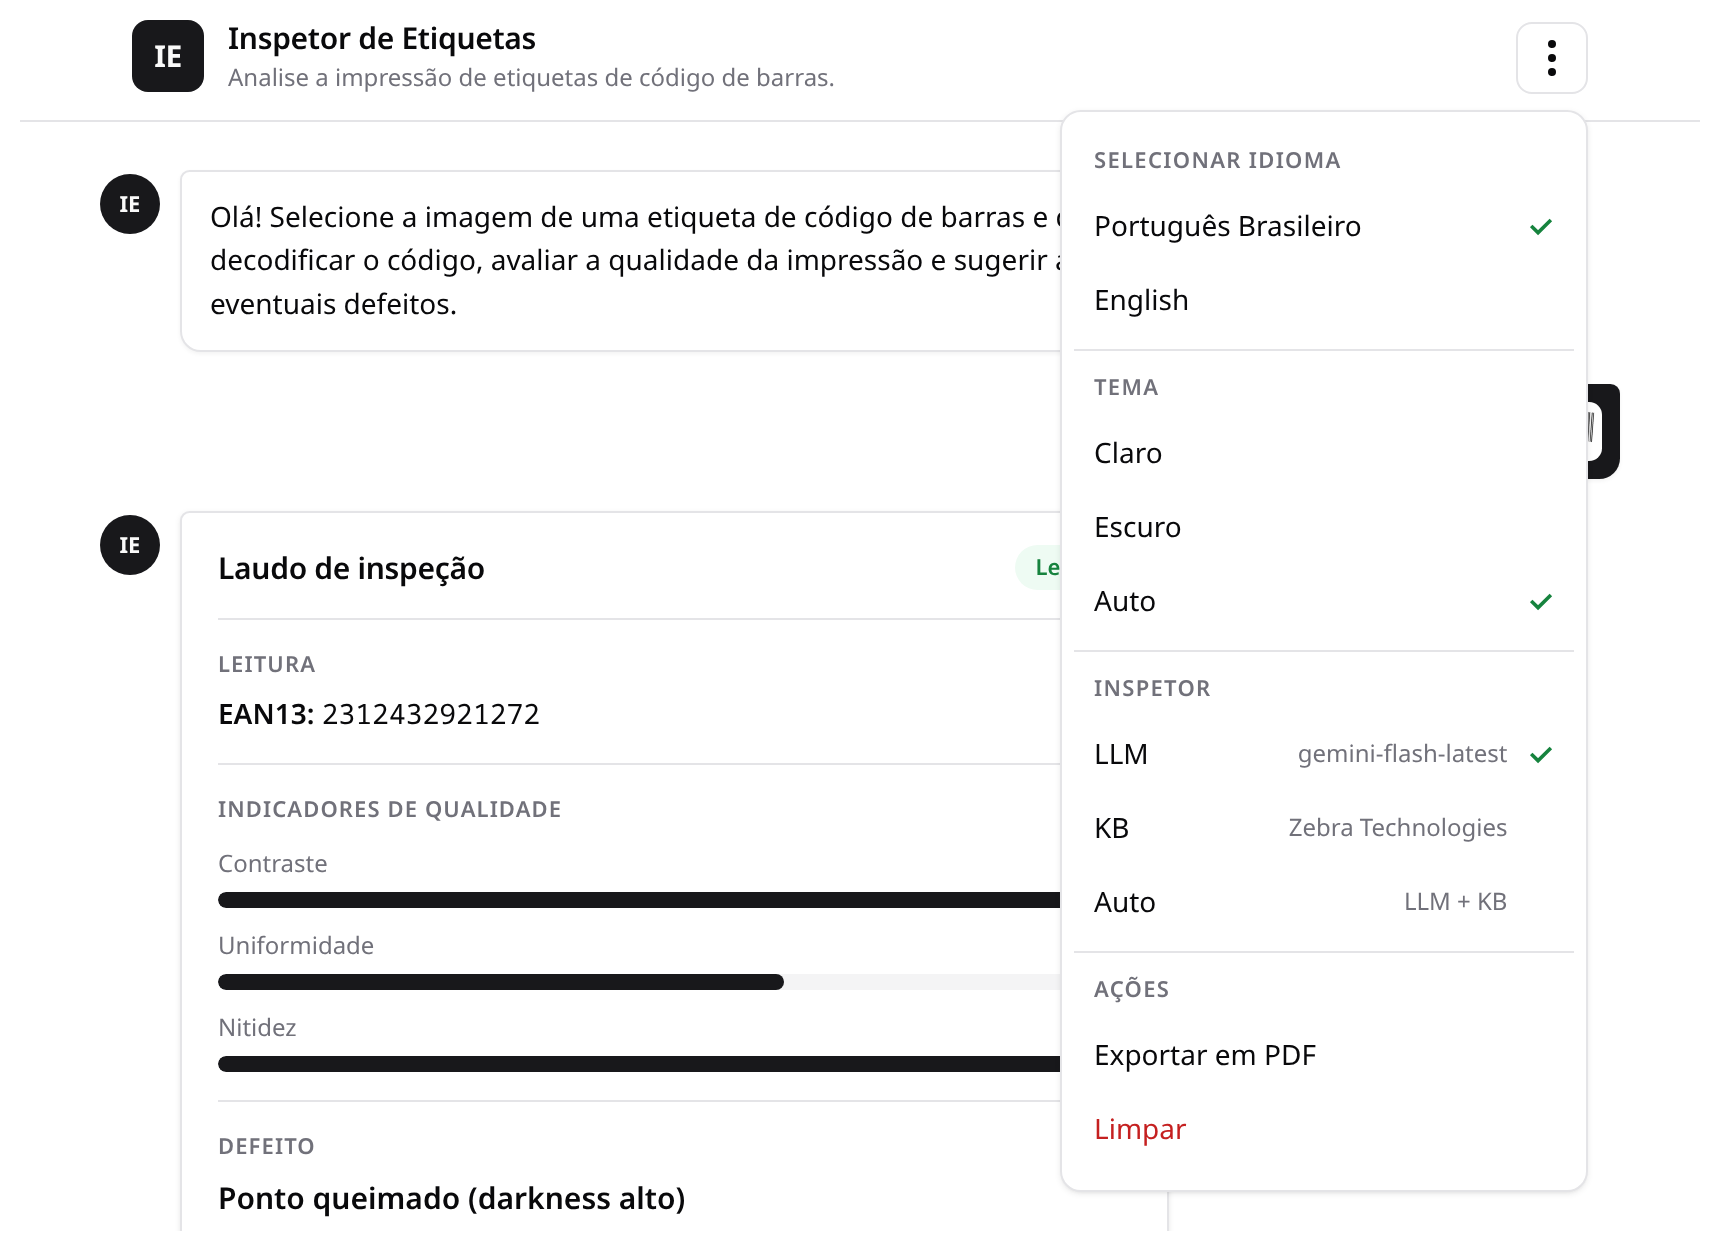
\includegraphics[width=0.62\textwidth]{figuras/chat_menu.png}

\vspace{2pt}
{\footnotesize Fonte: elaboração própria (2026).}
\end{figure}

% ---------------------------------------------------------------------------
\section{Resultados e discussão}\label{sec-resultados}
% ---------------------------------------------------------------------------

% NOTA: esta seção é um MODELO. Preencha com os seus experimentos. Não há
% números fabricados aqui — os traços (---) devem ser substituídos pelos
% valores obtidos.

\subsection{Configuração dos experimentos}

O experimento \textbf{E1 (classificação de defeitos)} foi executado sobre o conjunto
sintético (Seção~\ref{sec-dados}), dividido em 434 imagens de treino, 91 de validação
e 105 de teste (as sete classes com 15 amostras cada no teste). Empregou-se a CNN
\textbf{MobileNetV3-Small} inicializada com pesos do ImageNet e submetida a
\textit{fine-tuning} completo (\textit{backbone} descongelado) por 40 épocas, com
otimizador Adam (taxa de aprendizado $5\times10^{-4}$), perda de entropia cruzada e
lotes de 32 imagens; seleciona-se o melhor modelo pela acurácia de validação. Os
experimentos \textbf{E2} (concordância dos indicadores com uma referência) e
\textbf{E3} (multiagente \textit{versus} monolítico) dependem, respectivamente, de um
verificador/rótulo de referência e de uma chave do modelo LLM, permanecendo em
andamento (Seção~\ref{sec-baseline}).

\subsection{Resultados quantitativos}

Em uma execução real do sistema, a classificação de defeitos alcançou \textbf{acurácia
de 81,9\%} no conjunto de teste (105 imagens), com médias macro de precisão 0,85,
revocação 0,82 e F1 0,80. A Tabela~\ref{tab-metricas} detalha as métricas por classe.

\begin{table}[htb]
\centering
\caption{Métricas de classificação por classe (conjunto de teste sintético)}
\label{tab-metricas}
\begin{tabular}{@{}lcccc@{}}
\toprule
\textbf{Classe} & \textbf{Precisão} & \textbf{Revocação} & \textbf{F1} & \textbf{N}\\
\midrule
Sem defeito & 0,48 & 0,87 & 0,62 & 15\\
Cabeça queimada & 0,75 & 0,20 & 0,32 & 15\\
\textit{Ribbon} enrugado & 0,82 & 0,93 & 0,87 & 15\\
Ponto queimado & 1,00 & 1,00 & 1,00 & 15\\
Impressão clara & 1,00 & 1,00 & 1,00 & 15\\
Pressão desigual & 1,00 & 1,00 & 1,00 & 15\\
Cabeça suja & 0,92 & 0,73 & 0,81 & 15\\
\midrule
\textbf{Macro / total} & \textbf{0,85} & \textbf{0,82} & \textbf{0,80} & \textbf{105}\\
\bottomrule
\end{tabular}

\vspace{2pt}
{\footnotesize Fonte: elaboração própria (2026).}
\end{table}

A matriz de confusão (Tabela~\ref{tab-confusao}) esclarece o principal erro: as classes
\emph{sem defeito} e \emph{cabeça queimada} confundem-se mutuamente --- nesta execução,
11 das 15 etiquetas de \emph{cabeça queimada} foram classificadas como \emph{sem
defeito}. As finas zonas claras entre as barras de um código íntegro assemelham-se às
linhas brancas verticais do defeito de elemento da cabeça, o que rebaixa a revocação de
``cabeça queimada'' (0,20). As demais classes, de assinatura visual mais distinta, são
reconhecidas com F1 entre 0,81 e 1,00.

\begin{table}[htb]
\centering
\caption{Matriz de confusão no teste (linha: classe verdadeira; coluna: classe prevista)}
\label{tab-confusao}
\footnotesize
\begin{tabular}{@{}l ccccccc@{}}
\toprule
 & \rotatebox{90}{sem defeito~} & \rotatebox{90}{cab. queimada~} & \rotatebox{90}{\textit{ribbon} enrug.~} & \rotatebox{90}{ponto queim.~} & \rotatebox{90}{impr. clara~} & \rotatebox{90}{pressão desig.~} & \rotatebox{90}{cabeça suja~}\\
\midrule
Sem defeito             & 13 & 1 & 1  & 0  & 0  & 0  & 0\\
Cabeça queimada         & 11 & 3 & 1  & 0  & 0  & 0  & 0\\
\textit{Ribbon} enrugado & 0 & 0 & 14 & 0  & 0  & 0  & 1\\
Ponto queimado          & 0 & 0  & 0  & 15 & 0  & 0  & 0\\
Impressão clara         & 0 & 0  & 0  & 0  & 15 & 0  & 0\\
Pressão desigual        & 0 & 0  & 0  & 0  & 0  & 15 & 0\\
Cabeça suja             & 3 & 0  & 1  & 0  & 0  & 0  & 11\\
\bottomrule
\end{tabular}

\vspace{2pt}
{\footnotesize Fonte: elaboração própria (2026).}
\end{table}

Em testes ponta a ponta com o sistema em execução, o laudo é produzido por completo: o
código é decodificado (por exemplo, EAN-13 e EAN-8 lidos corretamente pela biblioteca
ZBar empacotada no projeto), o defeito é classificado e o diagnóstico traz a causa
provável e a correção --- para os defeitos de assinatura distinta, com confiança próxima
de 1,00.

\subsection{Multiagente \textit{versus} abordagem monolítica}\label{sec-baseline}

Esta é a comparação que transforma ``usei ADK'' em contribuição avaliável.
Reportar as mesmas métricas para a arquitetura decomposta e para uma abordagem
única (um só modelo/prompt fazendo tudo), discutindo confiabilidade, acerto por
classe, interpretabilidade do laudo e latência. \textbf{[A preencher.]}

\subsection{Análise e discussão}

O sistema mostrou-se eficaz para os defeitos de assinatura visual distinta --- ponto
queimado, impressão clara e pressão desigual atingiram F1 igual a 1,00, e \textit{ribbon}
enrugado (0,87) e cabeça suja (0,81) ficaram acima de 0,80. O ponto fraco concentra-se na
confusão mútua entre ``sem defeito'' e ``cabeça queimada'': as zonas claras entre as
barras de um código íntegro imitam as linhas brancas verticais do elemento danificado, de
modo que, dependendo do treino, uma das duas classes perde revocação. Isso evidencia a
necessidade de mais dados dessas classes e de um pós-processamento que combine a saída da
CNN com os indicadores de qualidade (por exemplo, exigir baixa uniformidade antes de
declarar dano na cabeça). Frente aos trabalhos da Seção~\ref{sec-relacionados}, que se
detêm na detecção do defeito, o diferencial aqui é acoplar a classificação a um
diagnóstico de causa fundamentado na documentação do fabricante.

\subsection{Limitações}

Ser explícito: os resultados acima são de um conjunto de teste \textbf{sintético e em
distribuição} (mesma geração do treino); a avaliação de generalização para defeitos
reais depende de um conjunto real --- por exemplo, das bases do \textit{Roboflow
Universe} citadas na Seção~\ref{sec-dados} --- e permanece em aberto. O treino de
defeitos apoia-se em dados sintéticos, com risco de \textit{domain gap}; a confusão entre
``sem defeito'' e ``cabeça queimada'' rebaixa a revocação de uma dessas classes (0,20
nesta execução); os números provêm de uma única execução de treino; a decodificação usa a
biblioteca ZBar, que o projeto empacota localmente (dispensando instalação no sistema),
embora códigos muito degradados ainda possam não ser lidos; o
conjunto de captura real é pequeno (52 imagens, apenas 1D); o sistema não é verificador
certificado (Seção~\ref{sec-qualidade}); e há dependência das condições de captura e da
generalização para outras impressoras/simbologias.

% ---------------------------------------------------------------------------
\section{Conclusão}\label{sec-conclusao}
% ---------------------------------------------------------------------------

% Redação provisória — revisar após os resultados.

Este trabalho propôs um sistema de detecção de defeitos de impressão em etiquetas
de códigos de barras que combina visão computacional e orquestração multiagente
(ADK), servido por uma API única para aplicativo e web, e que vai além da nota
tradicional ao sugerir a causa provável do defeito com base na documentação
técnica do fabricante. \textbf{[Sintetizar aqui a resposta à questão de pesquisa da
Seção~\ref{sec-metodo}, à luz dos resultados obtidos.]}

\noindent\textbf{Principais contribuições entregues:} \textbf{[retomar da
introdução as que se confirmaram]}.

\noindent\textbf{Trabalhos futuros:} ampliar o conjunto de dados com defeitos
reais; estender a símbolos 2D (Data Matrix/QR) via ISO/IEC 15415; aproximar os
indicadores estimados de um verificador certificado por calibração; otimizar a
latência da orquestração; e realizar avaliação em ambiente de produção.

% ===========================================================================
\postextual
% ===========================================================================

% ---------------------------------------------------------------------------
% REFERÊNCIAS
% ---------------------------------------------------------------------------
\bibliography{referencias}

\end{document}
